\documentclass[aoas,preprint]{imsart}

\RequirePackage[OT1]{fontenc}
\RequirePackage{amsthm,amsmath}
\RequirePackage[numbers]{natbib}
\RequirePackage[colorlinks,citecolor=blue,urlcolor=blue]{hyperref}

% settings
%\pubyear{2005}
%\volume{0}
%\issue{0}
%\firstpage{1}
%\lastpage{8}
\arxiv{arXiv:0000.0000}

\startlocaldefs
\numberwithin{equation}{section}
\theoremstyle{plain}
\newtheorem{thm}{Theorem}[section]
\endlocaldefs

\begin{document}

\begin{frontmatter}
%\title{Assessing Fox Mortality during Fox Hunting Trials\thanksref{T1}}
\runtitle{Fox Mortality}
%\thankstext{T1}{Footnote to the title with the ``thankstext'' command.}

\begin{aug}
\author{\fnms{First} \snm{Author}\thanksref{m1}\ead[label=e1]{first@somewhere.com}},
\author{\fnms{Second} \snm{Author}\thanksref{m1}\ead[label=e2]{second@somewhere.com}}


\thankstext{t1}{Some comment}
\runauthor{F. Author et al.}

\affiliation{Virginia Polytechnic Institute and State University\thanksmark{m1}}

\address{Address of the First and Second authors\\
Usually a few lines long\\
\printead{e1}\\
\phantom{E-mail:\ }\printead*{e2}}

\end{aug}

\begin{abstract}

Fox penning is a tradition whereby foxes are hunted with dogs in a large enclosed space. This is criticized by animal rights groups who claim that the practice is cruel. In this paper we investigate the factors that influence a fox's chances to survive in such pens and connect that to the notions of cruelty and of the fair chase. We then use our model to examine possible changes to fox penning policy and what effect those changes may have on fox survival. We conclude that by either allowing the foxes to acclimate to their environment or by limiting the number of hunting dogs in the pen, we can improve fox survival and recapture the spirit of the fair chase,

\end{abstract}

\begin{keyword}[class=MSC]
\kwd[Primary ]{60K35}
\kwd{60K35}
\kwd[; secondary ]{60K35}
\end{keyword}

\begin{keyword}
\kwd{sample}
\kwd{\LaTeXe}
\end{keyword}

\end{frontmatter}

\section{Introduction}

In this paper we talk about some motherfuckers(I) who think that what some other motherfuckers(II) is doing to some fuckin foxes is mean and shit. So we wanna know like what other shit can these motherfuckers(II) be doin different so that the motherfuckers(I) get off they case. Henceforth and towards that end, we procured data about the goings on of some fuckin foxes in a big ass pen, how many dogs they got, how long they been in there, and when they die so's that we can learn about what it is about this big ass pen that be killin the foxes. We do some Bayesian shit (normal data augmentation in a probit regression model to estimate a given's foxes survival probability on a given day) and run'd some dope ass code. Check it.

\section{Data}

Inferences are made from $P(\Theta|X,Y),$ where $
	\mathcal{X}=\left[
	\begin{array}{ll}
	X \\
	X^{*} 
	\end{array}
	\right]$ \\and $X^{*}$ denotes missing covariates. Then in a Bayesian paradigm $$P(\Theta|X,Y), = \int P(\Theta|X,X^{*},Y) p(X^{*}) dX^{*}.$$


\section{Model}

\begin{eqnarray}
y_{it} &\sim& Bernoulli(p_{it}) \\
probit(p_{it}) & = & \alpha + X_{t}\beta_{dogs} + \theta_{it} \\
\theta_{it} &\sim& N(\alpha_{i} + G_{it} \beta_{exp}, \phi^{-1})
\end{eqnarray}
where $i = \{1,...27\} $(fox), and $t= \{1,...,T\}$ (trials). The number of dogs for trial t is denoted $X_t$ and $G_{it}$ is the experience of fox $i$ on day $t$. Let $R_{it}$ be the risk matrix, where
\[
    R_{it}=\left\{
                \begin{array}{ll}
                  1 \quad \text{ if fox i is alive and collared on day t-1}\\
                  0 \quad \text{otherwise}
                \end{array}
              \right.
  \]
  We use data augmentation where 
  \begin{eqnarray}
  Z_{it} \sim N( \alpha + X_t\beta_{dogs} +\theta_{it})
  \end{eqnarray}
  and
\[
    Y_{it}=\left\{
                \begin{array}{ll}
                  1 \quad  Z_{it} > 0\\
                  0 \quad Z_{it} \leq 0
                \end{array}
              \right.
  \]
  
  
  \subsection{Outstanding Model Based Questions}
  \begin{itemize}
  \item Potential Interaction between experience and dogs
  \item how to handle non-trial deaths
  \begin{enumerate}
  \item exclude
  \item average dogs across week
  \item ???
  \end{enumerate}
  \item assess linearity of `XB' inside link function
  \item perhaps look at a comparison of the hazard (survival curve) for trial and non-trial days.
  \end{itemize}
  
\section{Results}


%\begin{figure}
%	\includegraphics[scale = .5]{survivalprob.pdf}
%\end{figure}


\begin{table}[h]
	%\caption{default}
	\begin{center}
		\begin{tabular}{|c|c|c|}
			\hline
			& mean & CI \\
			\hline
			$\alpha$ & 5.4 & (3.0,11.6) \\
			$\beta_{dogs}$ & -.008 & (-.015, -.004) \\
			$\beta_{exp}$ & -.65 & (-2.04,-.10) \\
			$\beta_{dogs*exp}$ & .0014 & (.0006, .0030)\\
			\hline
		\end{tabular}
	\end{center}
	\caption{Table of model coefficients.}
\end{table}

\paragraph{}To estimate our model parameters we ran a Gibbs sampler. The chain was run for 500,000 iterations with convergence happening rather quickly for all parameters. Estimates of the coefficients and 95\% credible intervals are give in table X. It can be seen that no credible interval contains 0, indicating that all predictors are useful. Interpretation of individual coefficients is complicated by the presence of the interaction term, but we can understand the model output by examining the heat map in figure X. We see that fox survival is lowest when there are many dogs and inexperienced foxes. This survival rises drastically as either the number of dogs drops or the experience of the foxes increases.

\subsection{Regime Changes}

\paragraph{}One of the motivating goals of this paper was to find ways to make fox penning less cruel. To learn about this, we considered how fox survival might change if the pens were to make policy changes. We considered four different situations:

	\begin{itemize}
		\item Regime A: No constraints on number of dogs or allotted acclimation time. This is currently in place.
		\item Regime B: Two weeks acclimation time with no dogs.
		\item Regime C: No more than 400 dogs allowed in pen at a time.
		\item Regime D: Two weeks acclimation time and 400 dog limit.
	\end{itemize}
These four regimes produced the following survival curves.

%\begin{figure}[h]
%	\begin{center}$
%		\begin{array}{cc}
%		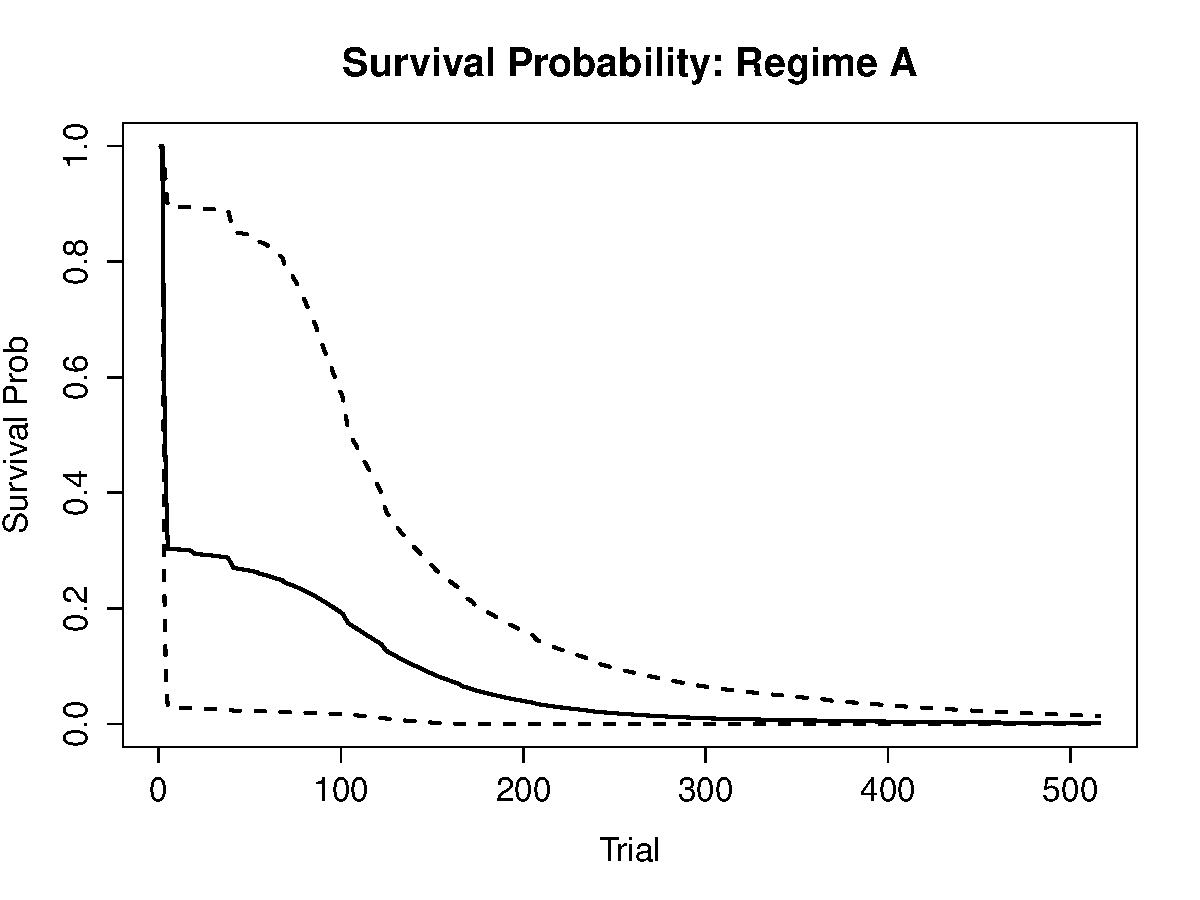
\includegraphics[width=3.4in]{RegA.pdf} & 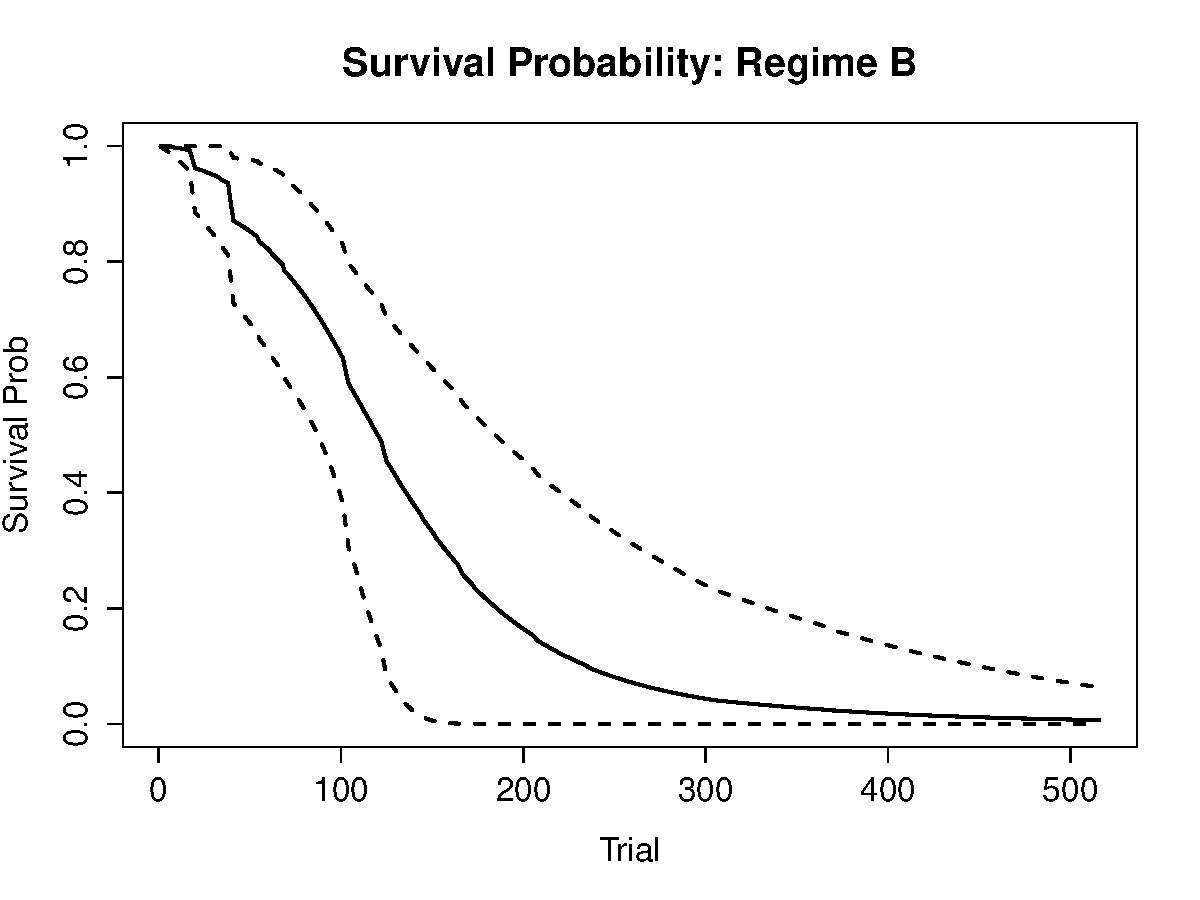
\includegraphics[width=3.4in]{RegB.pdf}\\
%		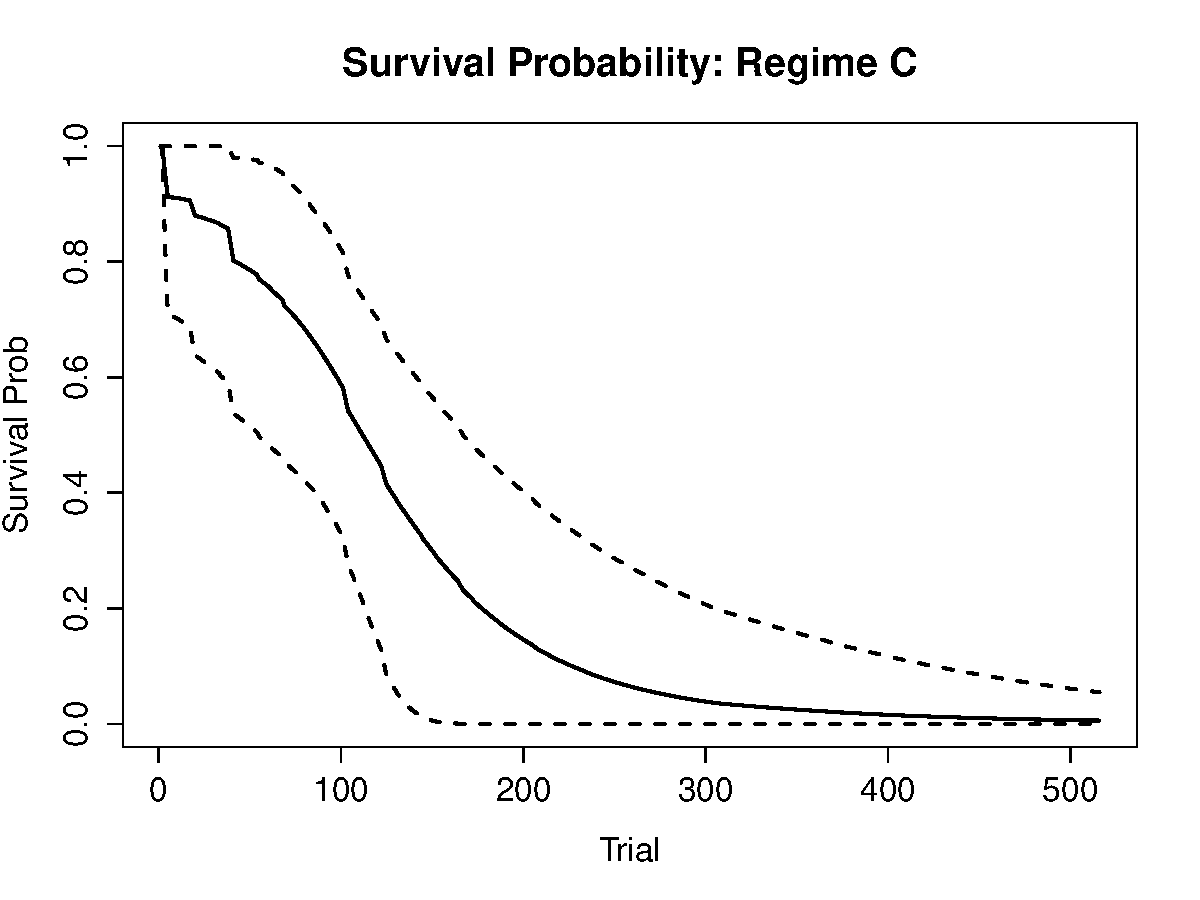
\includegraphics[width=3.4in]{RegC.pdf} & 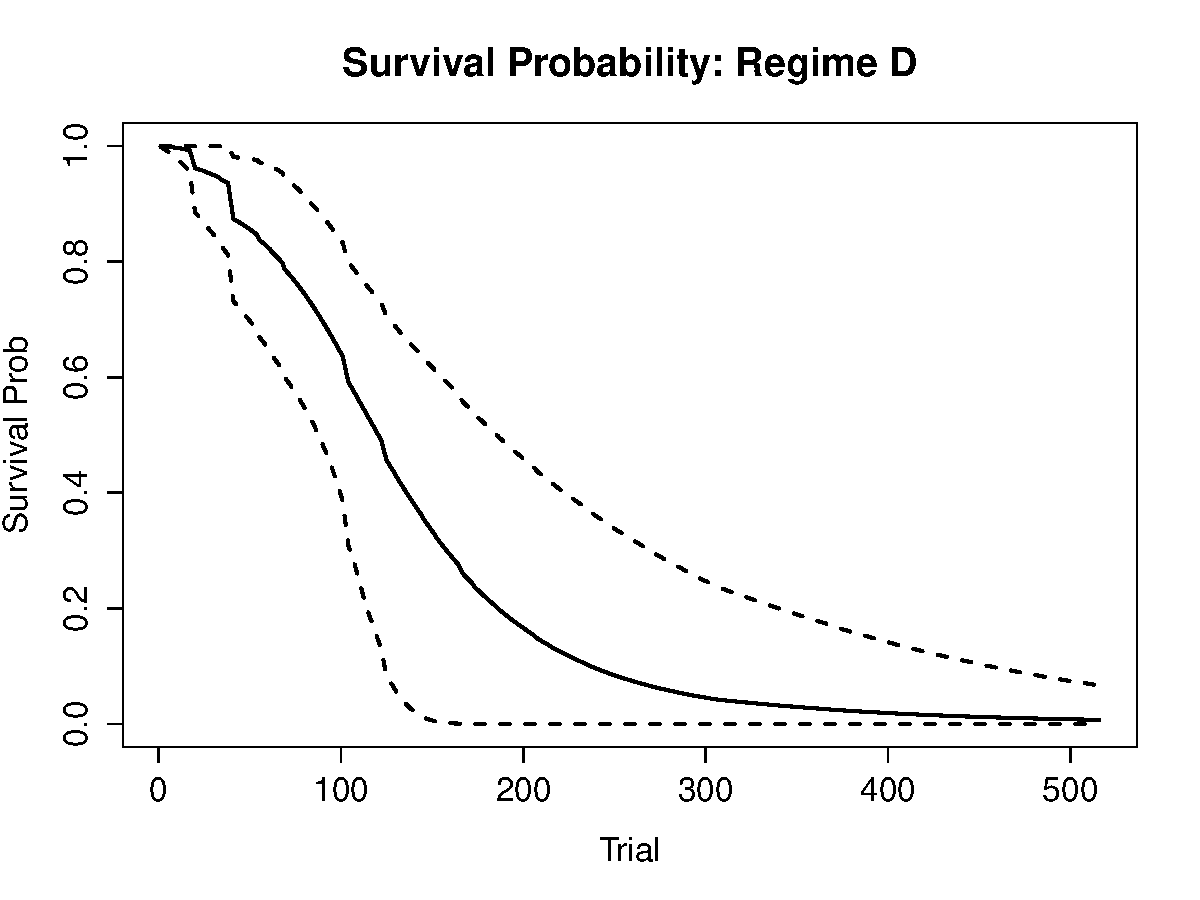
\includegraphics[width=3.4in]{RegD.pdf}
%		\end{array}$
%	\end{center}
%	\caption{Survival functions for the four regimes}
%	\label{fgr:1}
%\end{figure}
We see a precipitous drop in fox survival for regime A but not for any of the other three regimes. In fact, the other three plots look very similar.

\section{Discussion}

\paragraph{}While our analysis has been about fox survival, what we really wanted to learn about was cruelty. Indeed, it is not the intent of the pen that the fox should survive, but rather than the fox be given a fair chance at evasion in accordance with the concept of the fair chase. According to our analysis, fewer than half of the foxes survive beyond their first day under the current rules system. This can hardly be said to be a fair chase. Fortunately, it only takes a small change in policy to greatly improve fox survival. By either allowing the foxes acclimation time or by limiting the number of dogs in the pen we can eliminate the drastic fox mortality we see in the current regime and more closely align the practice of fox penning with the idea of the fair chase.













\begin{thebibliography}{9}

\bibitem{r1}
\textsc{Billingsley, P.} (1999). \textit{Convergence of
Probability Measures}, 2nd ed.
Wiley, New York.
\MR{1700749}


\end{thebibliography}

\end{document}
